\documentclass[a4paper,10pt,twocolumn]{article}
\usepackage[english]{babel}
\usepackage[style=ieee,backend=bibtex]{biblatex} \bibliography{ref.bib}
\usepackage[hidelinks]{hyperref}
\usepackage{fancyhdr}
\usepackage{float}
\usepackage{graphicx}
\usepackage[latin1]{inputenc}
\usepackage{nomencl}
\usepackage{mhchem}
\usepackage{multicol}
\usepackage{siunitx}
\usepackage{tikz}
    \usetikzlibrary{arrows}
    \usetikzlibrary{patterns}
    \usetikzlibrary{3d}
\usepackage{tikz-3dplot}
\usepackage{titling}
\usepackage{xspace}

\newcommand{\Comsol}{\textsc{Comsol}\xspace}
\newcommand{\comsol}{\textsc{comsol}\xspace}
\newcommand{\ComsolMultiphysics}{%
    \textsc{Comsol}~Multiphysics\textsuperscript{\textregistered}\xspace}
\newcommand{\Cmos}{\textsc{Cmos}\xspace}
\newcommand{\cmos}{\textsc{cmos}\xspace}
\newcommand{\Fem}{\textsc{Fem}\xspace}
\newcommand{\fem}{\textsc{fem}\xspace}
\newcommand{\Mems}{\textsc{Mems}\xspace}
\newcommand{\mems}{\textsc{mems}\xspace}

% Top matter
\title{\Mems Multimorph Capacitive Temperature Sensors in \ComsolMultiphysics}
\author{Z0966990}
\date{\today}

% Headers and footers
\pagestyle{fancy}
\fancyhf{}
\lhead{
\includegraphics[width=0.1\textwidth]{img/Durham.png}}
\chead{\thetitle}
\rhead{\theauthor}
\cfoot{\thepage}

\begin{document}

% Title and abstract
\thispagestyle{plain}

\twocolumn[{
\begin{@twocolumnfalse} \centering
    
\includegraphics[width=0.2\textwidth]{img/Durham.png}\\
    \Large\thetitle
    \vskip0.2em
    \large Level 3 Semiconductor, Physics and Devices\\
    \vskip0.4em
    \large\theauthor\\
    \vskip0.4em
    \large\thedate\\
    \hrulefill
    \renewcommand{\abstractname}{\large Abstract}
    \begin{abstract}
        This report describes how the $C$--$T$ characteristics of \mems
        multimorph capacitive temperature sensors vary with geometry, material
        choice and thermal-annealing temperature. The sensors were modelled
        using \fem and physics simulation software---\ComsolMultiphysics---so
        the key design choices for the model and mesh are also included.
    \end{abstract}
    \vskip\parsep
\end{@twocolumnfalse}
}]


\makenomenclature

% Acronyms
\nomenclature[A0]{\mems}{Microelectromechanical systems}

\printnomenclature

\section{Introduction}

In an increasingly data centric world with the number of sensors

\begin{figure}[h]
    \centering
    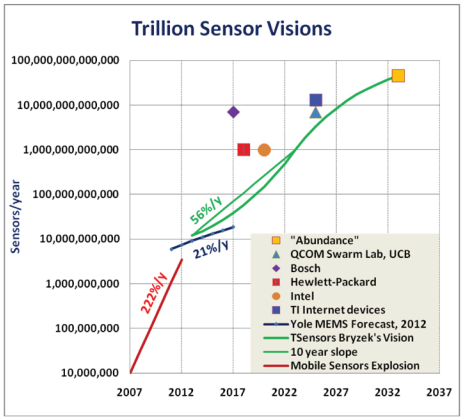
\includegraphics[width=0.4\textwidth]{img/trillion-sensors.png}
    \caption{Janusz Bryzek's trillion sensor vision~\.}
    \label{fig:tsensors}
\end{figure}

\emph{why sense temperature?}

\emph{what temperature sensors are available?}

\emph{why \mems?}

\section{Background}

\emph{what is a multimorph capacitor?}

\subsection{Construction}

\emph{how do we build an effective multimorph}

\emph{how do we make the sensor practical}

\subsection{Characterisation}

\emph{multimorph capacitance}

\emph{how do we characterise sensitivity?}

\emph{how do we characterise linearity?}

\section{Modelling}

\subsection{Geometry}

\emph{symmetry}

\begin{figure}[h]
    \centering
    \tdplotsetmaincoords{70}{110}
    \begin{small}
    \begin{tikzpicture}[scale=0.4\textwidth/0.800cm,tdplot_main_coords]

        % Substrate
        \begin{scope}[canvas is xy plane at z=0.190]
            \path [fill=lightgray!140] (0.000,0.000) -- (0.000,0.840) --
                (0.060,0.840) -- (0.060,0.000) -- (0.000,0.000);
            \draw [thin,dashed] (0.060/2,0.000) -- (0.060/2,0.840);
            \draw (0.060,0.000) -- (0.000,0.000) -- (0.000,0.840);
        \end{scope}
        \begin{scope}[canvas is xy plane at z=0.200]
            \path [fill=lightgray!140] (0.000,0.370) -- (0.000,0.470) --
                (0.060,0.470) -- (0.060,0.370) -- (0.000,0.370);
            \draw [thin,dashed] (0.000,0.840/2) -- (0.060,0.840/2);
            \draw (0.060,0.370) -- (0.000,0.370) -- (0.000,0.470);
        \end{scope}
        \begin{scope}[canvas is zx plane at y=0.470]
            \path [fill=lightgray!120] (0.190,0.000) -- (0.190,0.060) --
                (0.200,0.060) -- (0.200,0.000) -- (0.190,0.000);
            \draw [thin,dashed] (0.190,0.060/2) -- (0.200,0.060/2);
            \draw (0.190,0.000) -- (0.200,0.000);
        \end{scope}
        \begin{scope}[canvas is zx plane at y=0.840]
            \path [fill=lightgray!120] (0.000,0.000) -- (0.000,0.060) --
                (0.190,0.060) -- (0.190,0.000) -- (0.000,0.000);
            \draw [thin,dashed] (0.000,0.060/2) -- (0.190,0.060/2);
            \draw (0.190,0.000) -- (0.000,0.000) -- (0.000,0.060);
        \end{scope}
        \begin{scope}[canvas is yz plane at x=0.060]
            \path [fill=lightgray] (0.000,0.000) -- (0.840,0.000) -- 
                (0.840,0.190) -- (0.470,0.190) -- (0.470,0.200) --
                (0.370,0.200) -- (0.370,0.190) -- (0.000,0.190) --
                (0.000,0.000);
            \draw [thin,dashed] (0.840/2,0.000) -- (0.840/2,0.200);
            \draw (0.370,0.190) -- (0.370,0.200);
            \draw (0.840,0.000) -- (0.000,0.000) -- (0.000,0.190);
        \end{scope}

        % Beam
        \begin{scope}[canvas is xy plane at z=0.209]
            \path [fill=olive!140] (0.020,0.020) -- (0.020,0.820) --
                (0.040,0.820) -- (0.040,0.020) -- (0.020,0.020);
            \draw [thin,dashed] (0.020,0.840/2) -- (0.040,0.840/2);
            \draw [thin,dashed] (0.060/2,0.020) -- (0.060/2,0.820);
            \draw (0.040,0.020) -- (0.020,0.020) -- (0.020,0.820);
        \end{scope}
        \begin{scope}[canvas is zx plane at y=0.820]
            \path [fill=olive!120] (0.206,0.020) -- (0.206,0.040) -- 
                (0.209,0.040) -- (0.209,0.020) -- (0.206,0.020);
            \path [fill=cyan!120] (0.203,0.020) -- (0.203,0.040) -- 
                (0.206,0.040) -- (0.206,0.020) -- (0.203,0.020);
            \path [fill=magenta!120] (0.200,0.020) -- (0.200,0.040) -- 
                (0.203,0.040) -- (0.203,0.020) -- (0.200,0.020);
            \draw [thin,dashed] (0.200,0.060/2) -- (0.209,0.060/2);
            \draw (0.209,0.020) -- (0.200,0.020) -- (0.200,0.040);
        \end{scope}
        \begin{scope}[canvas is yz plane at x=0.040]
            \path [fill=olive] (0.020,0.206) -- (0.020,0.209) -- (0.820,0.209)
                -- (0.820,0.206) -- (0.020,0.206);
            \path [fill=cyan] (0.020,0.203) -- (0.020,0.206) -- (0.820,0.206) --
                (0.820,0.203)-- (0.020,0.203);
            \path [fill=magenta] (0.020,0.200) -- (0.020,0.203) -- (0.820,0.203)
                -- (0.820,0.200)-- (0.020,0.200);
            \draw [thin,dashed] (0.840/2,0.200) -- (0.840/2,0.209);
            \draw (0.820,0.200) -- (0.470,0.200);
            \draw (0.370,0.200) -- (0.020,0.200) -- (0.020,0.209);
        \end{scope}

        % Scale
        \draw [-serif cm] (0.200,0,0) -- ++(-0.050,0,0);
        \draw [-serif cm] (0.200,0,0) -- ++(0,0.050,0) 
            node[right]{\SI{50}{\micro\meter}};
        \draw [-serif cm] (0.200,0,0) -- ++(0,0,0.050);
    \end{tikzpicture}
    \end{small}
    \caption{Symmetry lines of the multimorph capacitive temperature
    sensor---marked with dashed lines.}
    \label{fig:cross-section}
\end{figure}


\emph{dimensions}

\begin{figure}[h]
    \centering
    \begin{small}
    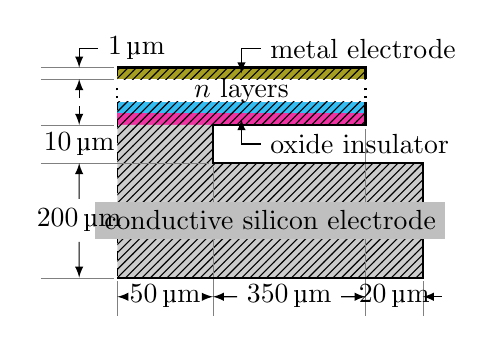
\begin{tikzpicture}[scale=0.4\textwidth/1cm]
        % Layers
        \path [fill=olive!80]   (0.20,0.72) rectangle (0.85,0.75);
        \path [fill=cyan!80]    (0.20,0.63) rectangle (0.85,0.66);
        \path [fill=magenta!80] (0.20,0.60) rectangle (0.85,0.63);
        \path [fill=lightgray!80] (0.20,0.20) -- (1.00,0.20) -- (1.00,0.50) -- 
            (0.45,0.50) -- (0.45,0.60) -- (0.20,0.60) -- (0.20,0.20);
        \path [pattern=north east lines] (0.20,0.72) rectangle (0.85,0.75);
        \path [pattern=north east lines] (0.20,0.63) rectangle (0.85,0.66);
        \path [pattern=north east lines] (0.20,0.60) rectangle (0.85,0.63);
        \path [pattern=north east lines] (0.20,0.20) -- (1.00,0.20) --  
            (1.00,0.50) -- (0.45,0.50) -- (0.45,0.60) -- (0.20,0.60) --
            (0.20,0.20);
        
        % Witness lines
        \draw [gray,ultra thin] (0.00,0.75) -- (0.19,0.75);
        \draw [gray,ultra thin] (0.00,0.72) -- (0.19,0.72);
        \draw [gray,ultra thin] (0.00,0.60) -- (0.19,0.60);
        \draw [gray,ultra thin] (0.00,0.50) -- (0.44,0.50);
        \draw [gray,ultra thin] (0.00,0.20) -- (0.19,0.20);

        \draw [gray,ultra thin] (0.20,0.10) -- (0.20,0.19);
        \draw [gray,ultra thin] (0.45,0.10) -- (0.45,0.49);
        \draw [gray,ultra thin] (0.85,0.10) -- (0.85,0.59);
        \draw [gray,ultra thin] (1.00,0.10) -- (1.00,0.19);

        % Outline
        \draw [thick] (0.20,0.20) -- (1.00,0.20) -- (1.00,0.50) -- (0.45,0.50)
            -- (0.45,0.60) -- (0.85,0.60) -- (0.85,0.66);
        \draw [dotted,thick] (0.85,0.67) -- (0.85,0.71);
        \draw [thick] (0.85,0.72) -- (0.85,0.75) -- (0.20,0.75);
        \draw [dashed] (0.20,0.75) -- (0.20,0.72);
        \draw [dotted,thick] (0.20,0.67) -- (0.20,0.71);
        \draw [dashed] (0.20,0.66) -- (0.20,0.20);

        % Labels
        \node [right] at (0.575,0.80) {metal electrode};
        \draw [latex-] (0.525,0.735) -- (0.525,0.80) -- (0.575,0.80);
        \node at (0.525,0.69) {$n$ layers};
        \draw [latex-] (0.525,0.615) -- (0.525,0.55) -- (0.575,0.55);
        \node [right] at (0.575,0.55) {oxide insulator};
        \node [align=center,fill=lightgray] at (0.60,0.35)
            {conductive silicon electrode};

        % Dimensions
        \node [right] at (0.15,0.80) {\SI{1}{\micro\meter}};
        \draw [latex-] (0.10,0.75) -- (0.10,0.80) -- (0.15,0.80);
        \node at (0.10,0.55) {\SI{10}{\micro\meter}};
        \draw [-latex] (0.10,0.67) -- (0.10,0.72);
        \draw [latex-] (0.10,0.60) -- (0.10,0.65);
        \node (d1) at (0.10,0.35) {\SI{200}{\micro\meter}};
        \draw [-latex] [above] (d1) -- (0.10,0.50);
        \draw [-latex] [below] (d1) -- (0.10,0.20);

        \node (d2) at (0.325,0.15) {\SI{50}{\micro\meter}};
        \draw [-latex] [left] (d2)-- (0.20,0.15);
        \draw [-latex] [right] (d2) -- (0.45,0.15);
        \node (d3) at (0.65,0.15) {\SI{350}{\micro\meter}};
        \draw [-latex] [left] (d3) -- (0.45,0.15);
        \draw [-latex] [right] (d3) -- (0.85,0.15);
        \draw [latex-] (1.00,0.15) -- (1.05,0.15);
        \node at (0.925,0.15) {\SI{20}{\micro\meter}};
    \end{tikzpicture}
    \end{small}
    \caption{Cross-section of the multimorph temperature sensor---not to scale.}
    \label{fig:cross-section}
\end{figure}

\emph{mesh}

\subsection{Materials}
\subsection{Physics}

\section{Results}
\section{Analysis}
\section{Conclusion}

\printbibliography

\end{document}